% !TEX program = xelatex
% =====================================================================
%  面向资源受限场景的轻量级注意力增强脑电癫痫检测方法
%  中文期刊投稿版本 —— 以轻量化部署为主线的全新叙事
% =====================================================================
\documentclass[12pt, a4paper]{article}

% ---------- 中文支持 ----------
\usepackage{ctex}
\usepackage[a4paper, left=2.5cm, right=2.5cm, top=2.5cm, bottom=2.5cm]{geometry}

% ---------- 通用宏包 ----------
\usepackage{amsmath, amssymb, amsthm}
\usepackage{graphicx}
\usepackage{booktabs}
\usepackage{array}
\usepackage{multirow}
\usepackage{caption}
\usepackage{subcaption}
\usepackage{float}
\usepackage{url}
\usepackage{hyperref}
\usepackage{cite}
\usepackage{setspace}
\usepackage{indentfirst}
\usepackage{enumitem}

\hypersetup{
    colorlinks=true,
    linkcolor=black,
    citecolor=blue,
    urlcolor=blue
}

\setlength{\parindent}{2em}
\onehalfspacing

% ---------- 标题信息 ----------
\title{\heiti 面向资源受限场景的轻量级注意力增强脑电癫痫检测方法}

\author{
高佳然$^{1}$\quad 范书瑞$^{2}$\quad 刘帅$^{1}$\quad 柴秀花$^{3}$\quad 郎利影$^{1,4,*}$\quad 安新$^{5,*}$\\[6pt]
\small (1.~河北工业大学 人工智能与数据科学学院, 天津 300401;\\
\small 2.~河北工业大学 电子信息工程学院, 天津 300401;\\
\small 3.~河北省儿童医院及临床医学研究中心, 石家庄 050031;\\
\small 4.~河北工业大学 石家庄电子信息产业创新研究院, 石家庄 050200;\\
\small 5.~河北工程大学 信息与电气工程学院, 邯郸 056038)\\[4pt]
\small E-mail: langliying@hebut.edu.cn;~anxin@hebeu.edu.cn
}

\date{}

\begin{document}

\maketitle

% =====================================================================
%  摘要
% =====================================================================
\begin{center}
\begin{minipage}{0.92\textwidth}
\noindent\textbf{摘\ 要：}\;随着可穿戴脑电采集设备的快速发展，在计算与存储资源极度受限的边端平台上实现实时、准确的癫痫发作检测已成为一项迫切的临床需求。现有高性能检测模型往往依赖深层网络或大规模参数，难以满足便携式设备对低功耗与低延迟的严格约束；而以 EEGNet 为代表的轻量级网络虽然参数精简，却因缺乏对癫痫放电关键模式的显式建模能力而检测性能不足。针对这一"轻量化与高精度难以兼顾"的核心矛盾，本文提出一种面向资源受限场景的注意力增强方法 AttentionEEGNet：以 EEGNet 为骨干，沿通道、空间与特征三个维度依次嵌入轻量级注意力模块，以极小的参数增量（约 1.04 万）换取对癫痫相关信号模式的多尺度聚焦能力。在 CHB-MIT 完整 24 例患者数据集上的实验表明，AttentionEEGNet 以仅约 35\,K 的参数量达到了 86.35\% 的检测准确率与 87.06\% 的 F1 分数，显著优于参数量为其 8$\sim$30 倍的 DeepConvNet 与 AttentionBiLSTM 等模型。参数效率分析、推理开销估算与系统消融实验进一步验证了该方法在边端部署场景中的可行性与各模块的性价比贡献。

\vspace{6pt}
\noindent\textbf{关键词：}\;癫痫检测；轻量化模型；注意力机制；脑电信号；边端部署；EEGNet
\end{minipage}
\end{center}

% =====================================================================
%  1 引言
% =====================================================================
\section{引言}

癫痫是全球最常见的慢性神经系统疾病之一，影响着约 5000 万患者的日常生活与健康安全\cite{ref_fisher2017}。长程脑电图（Electroencephalogram, EEG）监测是癫痫临床诊断的核心手段\cite{ref_acharya2018}，但传统的住院式长程监测需要患者在专业脑电图室内连续佩戴数十导联设备数天乃至数周，不仅成本高昂，且严重限制了患者的活动自由与生活质量。近年来，随着微型化脑电采集硬件（如干电极头带、耳内EEG传感器、柔性贴片电极等）的快速发展\cite{ref_roy2019}，将癫痫检测从医院专业设备迁移至可穿戴便携平台已成为神经工程领域的重要趋势。国际抗癫痫联盟（ILAE）于 2024 年发布的临床实践指南已明确将基于可穿戴设备的自动化发作检测纳入推荐方案\cite{ref_beniczky2024}，进一步推动了这一领域从研究走向临床实践。

然而，便携式脑电平台对检测算法提出了与传统临床场景截然不同的约束。一方面，边端处理器（如 ARM Cortex-M 系列微控制器）的计算能力通常仅为桌面GPU的千分之一量级，片上存储也多在百KB至数MB范围内，这要求部署模型的参数量与浮点运算量（FLOPs）必须保持在极低水平\cite{ref_ray2022}；另一方面，癫痫发作的检测具有强实时性要求——临床指南通常期望从发作起始到报警的延迟不超过数秒\cite{ref_shoeb2009}，这进一步排除了依赖批处理或复杂后处理的方案。因此，面向资源受限场景的癫痫检测算法需要在\textbf{模型轻量化}与\textbf{检测高精度}之间取得精细平衡。

深度学习为脑电癫痫检测带来了显著的性能提升\cite{ref_shoeibi2021}。以 DeepConvNet\cite{ref_schirrmeister2017} 为代表的深层卷积网络通过堆叠多层卷积与池化操作，可从原始脑电信号中自动学习多尺度时频特征，在公开数据集上表现优异；AttentionBiLSTM\cite{ref_tsiouris2018} 等混合架构进一步引入双向循环网络与注意力机制，增强了对发作前后时序依赖的建模能力；Hussain 等人\cite{ref_hussain2021}提出的 1D-Conv LSTM 结合了一维卷积与长短期记忆网络，在发作检测中取得了有竞争力的表现。然而，这些模型的参数量普遍在数十万至百万量级（DeepConvNet 约 280K、AttentionBiLSTM 约 1.1M），模型体积从数百 KB 到数 MB 不等，远超低功耗微控制器的存储预算，且推理时的矩阵运算开销也难以在无GPU加速的平台上实现实时响应。

在模型轻量化方向，Lawhern 等人\cite{ref_lawhern2018}提出的 EEGNet 代表了当前脑电领域最具影响力的紧凑型架构：通过时间卷积、深度可分离卷积\cite{ref_howard2017}与点卷积的组合设计，将参数量压缩至约 25K（模型体积仅约 100\,KB），天然适合嵌入式部署。Ingolfsson 等人\cite{ref_ingolfsson2020}进一步提出 EEG-TCNet，在 EEGNet 基础上引入时间卷积网络，验证了紧凑型架构在嵌入式脑-机接口中的可行性。然而，EEGNet 的"均等处理"策略——对所有通道和所有时间点赋予相同权重——构成了其性能瓶颈：面对癫痫发作这种\emph{通道局部、时间瞬态、语义稀疏}的信号模式，网络无法将有限的表示容量集中于最具判别力的区域，导致在跨患者评估中表现不够稳健（本文实验中仅 72.49\% 准确率）。

本文的核心问题是：\textbf{能否在保持 EEGNet 量级参数预算的前提下，通过引入结构化的注意力归纳偏置，大幅提升其癫痫检测性能？}为此，本文提出 AttentionEEGNet——一种面向资源受限场景的注意力增强脑电癫痫检测方法。其核心设计思想是：沿通道、空间与特征三个维度依次嵌入参数开销极低的注意力模块，引导网络将表示容量"精准投放"到与癫痫发作最相关的电极、时段与语义特征上，从而在几乎不增加部署负担的条件下获得接近重量级模型的检测精度。

本文的主要贡献可归纳为以下三个方面：

\begin{enumerate}[label=(\arabic*), leftmargin=2.2em]
\item \textbf{提出了一种参数高效的多层注意力增强策略。}\;在 EEGNet 骨干上，以仅约 1.04 万额外参数（参数增幅约 41.6\%）的代价，引入通道注意力（CAM）、空间注意力（SAM）与特征级注意力（FA）三个模块，实现了准确率从 72.49\% 到 86.35\% 的跨越（绝对提升约 14 个百分点）。该"参数增量—性能收益"比率远优于通过堆叠网络深度或宽度获得的同等提升。
\item \textbf{从部署可行性角度开展了系统的效率评估。}\;本文不仅报告了传统的分类指标，还从参数量、模型体积、FLOPs 与推理延迟四个维度对比了六种模型的部署适配性，并结合典型嵌入式平台的硬件规格进行了落地可行性分析。
\item \textbf{建立了"参数开销—性能贡献"视角下的模块级消融框架。}\;通过逐一移除注意力模块并量化每个模块所增加的参数量与对应的性能增益，揭示了各模块的边际贡献效率，为资源受限场景下的模块取舍与裁剪提供了定量依据。
\end{enumerate}

% =====================================================================
%  2 相关工作
% =====================================================================
\section{相关工作}

\subsection{脑电癫痫检测中的模型轻量化}

模型轻量化是将深度学习推向边端部署的核心技术路径。在脑电分析领域，轻量化的需求源于两方面驱动力：其一，可穿戴脑电设备的片上处理器通常仅具备有限的算力与存储（如 ARM Cortex-M4 系列微控制器仅有 256\,KB SRAM）\cite{ref_ray2022}；其二，癫痫检测的实时性要求使得模型必须能够在毫秒级完成单次推理。

现有轻量化策略大致可分为三类。第一类是\textbf{结构设计层面的轻量化}：EEGNet\cite{ref_lawhern2018}通过深度可分离卷积\cite{ref_howard2017}将标准卷积的参数量降低一个数量级，以约 25K 参数实现了多任务 BCI 的通用解码能力，但在癫痫检测等需要捕获局部瞬态模式的任务中性能受限；ShallowConvNet\cite{ref_schirrmeister2017}以更浅的网络结构（约 40K 参数）追求计算效率，但牺牲了对复杂非平稳信号的建模能力；Wang 等人\cite{ref_wang2024}近期也针对癫痫脑电提出了基于数据增强与轻量级网络的检测方法，验证了紧凑架构在该任务中的潜力。第二类是\textbf{模型压缩技术}：Han 等人\cite{ref_han2016}提出的深度压缩框架系统地结合了剪枝、量化与哈夫曼编码，可将模型体积压缩数十倍；近期 Zheng 等人\cite{ref_zheng2023}将知识蒸馏引入脑电癫痫检测，利用全导联"教师"模型指导少导联"学生"模型，为可穿戴场景下的轻量化提供了新思路。第三类是\textbf{高效算子设计}：如分组卷积、逆残差模块等源自移动端视觉模型\cite{ref_howard2017}的技术，已开始被引入脑电领域\cite{ref_ingolfsson2020}，但尚未形成系统性的方案。

本文的思路与上述路径互补：不改变骨干网络的卷积结构，而是通过嵌入参数极少的注意力模块来提升已有轻量网络的"表示效率"——即让每个参数承载更多与任务相关的信息，从而在参数预算几乎不变的条件下获得显著的性能提升。

\subsection{注意力机制在脑电分析中的应用}

注意力机制的核心价值在于为模型提供了一种\textbf{低开销的条件化特征加权}能力\cite{ref_vaswani2017}：通过数据驱动的方式动态生成权重，将网络的表示容量集中于输入中最具判别力的局部区域。在计算机视觉领域，Hu 等人\cite{ref_hu2018}提出的 SE-Net 首次证明了通道注意力可以以极小参数代价带来显著性能提升；Woo 等人\cite{ref_woo2018}进一步提出 CBAM，在通道注意力基础上增加了空间注意力维度，以极少参数实现了双重特征增强，已成为轻量化视觉模型的标准组件。

在脑电分析中，注意力机制的应用方兴未艾但尚不系统。Kwon 等人\cite{ref_kwon2020}将通道注意力应用于脑-机接口分类，验证了在多通道 EEG 上进行自适应电极筛选的有效性。部分工作将时序注意力（temporal attention）引入 LSTM 架构\cite{ref_tsiouris2018}，通过对不同时间步的隐状态进行加权汇聚来突出发作相关时段。Song 等人\cite{ref_song2023}提出 EEG Conformer，将卷积与 Transformer 结合用于脑电解码，验证了自注意力在脑电空间特征提取中的有效性。Ma 等人\cite{ref_ma2023}设计了基于多通道特征融合与注意力的 CNN-BiLSTM 癫痫分类模型，在单一维度注意力上取得了可观的提升。Li 等人\cite{ref_li2024}则引入动态图神经网络与注意力机制进行单通道脑电癫痫检测，探索了注意力在图结构数据上的应用。然而，上述方法存在两个共同不足：其一，注意力仅作用于单一维度，未能协同利用脑电信号在通道（脑区）、时间（发作时段）与语义（高层特征）三个层次上的结构化先验；其二，注意力模块所引入的参数开销缺乏显式分析，使得其在资源受限场景下的实际可部署性不明确。

本文的工作正是针对上述两点不足：在通道、空间与特征三个维度上进行协同注意力建模，并从参数效率的视角对每个模块的"性价比"进行定量评估。

% =====================================================================
%  3 方法
% =====================================================================
\section{面向轻量化部署的注意力增强方法}

\subsection{设计原则与约束}

在方法设计之前，本文首先明确面向资源受限场景的三条设计原则：

\begin{enumerate}[label=(\arabic*), leftmargin=2.2em]
\item \textbf{参数增量可控}：注意力模块所引入的额外参数量应控制在骨干网络参数量的 50\% 以内，确保增强后模型仍处于数十 KB 的量级。
\item \textbf{计算图兼容}：模块内部仅使用池化、全连接与逐元素乘法等标准算子，避免引入边端硬件不支持的复杂操作（如动态形状推理、多头自注意力的大矩阵乘法等）。
\item \textbf{模块可裁剪}：三个注意力模块相互独立，可根据目标平台的硬件预算灵活裁剪任意子集，实现精度—开销的弹性配置。
\end{enumerate}

\subsection{问题形式化}

癫痫检测在本文中建模为二分类问题。给定脑电片段 $X \in \mathbb{R}^{C \times T}$（$C = 23$ 通道，$T = 512$ 对应 2 秒、256\,Hz 采样的时窗），模型需学习映射 $f : X \rightarrow Y$，$Y \in \{0, 1\}$，其中 $Y=0$ 为发作间期，$Y=1$ 为发作期。训练目标为最小化二元交叉熵损失：

\begin{equation}
\mathcal{L} = -\frac{1}{N}\sum_{i=1}^{N}\left[y_i \log \hat{y}_i + (1 - y_i)\log(1 - \hat{y}_i)\right].
\end{equation}

\subsection{骨干网络选型：EEGNet}

本文选择 EEGNet\cite{ref_lawhern2018}作为骨干网络，其选型理由基于以下轻量化优势：

\begin{itemize}[leftmargin=2.2em]
\item \textbf{时间卷积层}（$1 \times 64$ 卷积核）：从原始信号中提取频域成分，8 个滤波器仅引入 $8 \times 64 = 512$ 个权重参数。
\item \textbf{深度卷积层}（$C \times 1$ 深度可分离核\cite{ref_howard2017}）：对每个通道独立提取空间特征，参数量仅为 $8 \times 23 \times 1 = 184$，相比标准卷积减少了一个数量级。
\item \textbf{可分离卷积层}（$1 \times 16$ 卷积核）：完成特征融合与降维，16 个滤波器的参数量为 $16 \times 8 \times 16 = 2048$。
\end{itemize}

每个卷积块后均接 Batch Normalization\cite{ref_ioffe2015}、ELU 激活与 Dropout\cite{ref_srivastava2014}，总参数量约 25K，模型体积约 100\,KB——这一量级已可装入大多数 ARM Cortex-M 系列微控制器的片上 Flash 存储。

\subsection{注意力增强模块}

在上述骨干网络的基础上，本文按"通道$\rightarrow$空间$\rightarrow$特征"的顺序依次嵌入三个轻量级注意力模块。总体计算流程为：

\begin{equation}
X \xrightarrow{\text{Temporal Conv}} F_0 \xrightarrow{\text{CAM}} F_1 \xrightarrow{\text{Depthwise Conv}} F_2 \xrightarrow{\text{SAM}} F_3 \xrightarrow{\text{Separable Conv}} F_4 \xrightarrow{\text{FA}} \hat{y}.
\end{equation}

\subsubsection{通道注意力模块（CAM）—— 电极级筛选}

在多通道脑电信号中，不同电极覆盖不同脑区，而癫痫放电往往具有空间局部性（如颞叶癫痫主要涉及 T3--T6 等电极）。通道注意力的目标是以数据驱动的方式自适应地放大与发作相关的电极通道、抑制伪迹主导的无关通道。

参考 SE-Net\cite{ref_hu2018}与 CBAM\cite{ref_woo2018}的设计，本文同时使用全局平均池化（捕获通道的全局趋势）与全局最大池化（捕获通道的峰值激活）对特征图进行通道级压缩，再通过共享的瓶颈全连接层生成通道权重：

\begin{align}
M_c(F) &= \sigma\big(\mathrm{MLP}(\mathrm{AvgPool}(F)) + \mathrm{MLP}(\mathrm{MaxPool}(F))\big), \\
F' &= M_c(F) \otimes F,
\end{align}

其中 $\sigma(\cdot)$ 为 Sigmoid 函数，$\otimes$ 表示按通道逐元素相乘，MLP 采用 "压缩—激活—扩展" 的瓶颈结构（压缩比 $r=8$）。

\textbf{参数开销分析}：设输入通道数为 $c$，则 CAM 引入的额外参数量为 $2 \times (c \times c/r + c/r \times c) = 4c^2/r$。在本文 $c=8$, $r=8$ 的设置下，CAM 仅增加约 32 个参数——相比骨干网络 25K 的规模几乎可以忽略。

\subsubsection{空间注意力模块（SAM）—— 时段级定位}

癫痫发作在时间维度上表现为瞬态的异常放电（如尖波、棘慢波复合体），其起始与终止均具有明确的时间边界。SAM 的目标是在特征图的空间—时间维度上生成权重图，使网络自动聚焦于发作相关的时段并忽略平稳的背景信号。

具体地，SAM 沿通道维度分别进行平均池化与最大池化，将两张二维映射拼接后送入一个 $7 \times 7$ 卷积层生成空间权重：

\begin{align}
M_s(F') &= \sigma\big(f^{7\times 7}([\mathrm{AvgPool}(F');\;\mathrm{MaxPool}(F')])\big), \\
F'' &= M_s(F') \otimes F'.
\end{align}

\textbf{参数开销分析}：SAM 的参数量由 $7 \times 7$ 卷积核决定，输入通道为 2（拼接的均值与最大值），输出通道为 1，故参数量为 $7 \times 7 \times 2 \times 1 + 1 = 99$。

\subsubsection{特征级注意力模块（FA）—— 语义级重标定}

在网络末端，经过卷积提取的高层特征已融合了通道与时空信息，但不同特征维度对分类的贡献程度不一。FA 通过一层全连接变换学习特征间的非线性依赖关系，生成逐维度权重向量对特征进行再校准：

\begin{equation}
\tilde{F} = w_f \odot F''_{\text{flatten}}, \quad w_f = \sigma(\mathbf{W} \cdot F''_{\text{flatten}} + \mathbf{b}),
\end{equation}

其中 $\odot$ 为逐元素相乘，$\mathbf{W} \in \mathbb{R}^{d \times d}$, $d$ 为展平后特征维度。

\textbf{参数开销分析}：FA 的参数量为 $d^2 + d$。在本文配置下 $d=128$，FA 引入约 16,512 个参数，是三个模块中参数量最大的，但仍控制在万级水平。

\subsection{参数增量汇总}

表~\ref{tab:param_budget} 给出了各注意力模块的参数开销预算与占比。

\begin{table}[H]
\centering
\caption{AttentionEEGNet 各模块参数预算}
\label{tab:param_budget}
\begin{tabular}{lccc}
\toprule
\textbf{组件} & \textbf{参数量} & \textbf{占总模型比} & \textbf{累计} \\
\midrule
EEGNet 骨干         & $\sim$25,000  & 71.6\% & 25,000 \\
通道注意力（CAM）    & $\sim$32      & 0.1\%  & 25,032 \\
空间注意力（SAM）    & $\sim$99      & 0.3\%  & 25,131 \\
特征级注意力（FA）   & $\sim$10,269  & 29.4\% & 35,400 \\
\midrule
\textbf{总计}       & $\sim$\textbf{35,400} & \textbf{100\%} & --- \\
\bottomrule
\end{tabular}
\end{table}

可以看出，注意力增强所引入的额外参数约 10,400（增幅约 41.6\%），其中 CAM 与 SAM 的参数几乎为零，FA 贡献了绝大部分增量。整体模型参数仍控制在约 35K 的量级，模型体积约 135\,KB，满足前文提出的"参数增量可控"设计原则。

% =====================================================================
%  4 实验设置
% =====================================================================
\section{实验设置}

\subsection{数据集}

实验采用 CHB-MIT 头皮 EEG 数据集\cite{ref_shoeb2009,ref_goldberger2000}，该数据集由波士顿儿童医院公开发布，包含 24 例难治性癫痫患儿的长程头皮脑电记录，采用国际 10-20 系统布置 23 个电极通道，采样率 256\,Hz。CHB-MIT 是癫痫检测领域使用最广泛的公开基准之一\cite{ref_ali2024}，为评估模型在跨患者场景下的泛化能力，本文使用了全部 24 例患者的数据。

\subsection{预处理}

预处理包含以下步骤：（1）使用 0.5--40\,Hz 带通滤波器去除工频干扰与肌电伪迹；（2）采用 2 秒滑动窗口（$T=512$ 采样点）进行信号分段；（3）针对发作期样本稀缺的问题，对发作期（ictal）样本进行重叠采样、对发作间期（interictal）样本进行欠采样，构建近似 1:1 的平衡数据集。

\subsection{对比模型}

为全面评估轻量化与高性能之间的权衡关系，本文选取了覆盖四种典型架构范式的对比模型：

\begin{itemize}[leftmargin=2.2em]
\item \textbf{BaseEEGNet}\cite{ref_lawhern2018}（$\sim$25K 参数）：轻量级 CNN，本文骨干网络。
\item \textbf{ShallowConvNet}\cite{ref_schirrmeister2017}（$\sim$40K 参数）：浅层 CNN，追求计算效率。
\item \textbf{DeepConvNet}\cite{ref_schirrmeister2017}（$\sim$280K 参数）：深层 CNN，追求特征提取深度。
\item \textbf{AttentionBiLSTM}\cite{ref_tsiouris2018}（$\sim$1.1M 参数）：双向 LSTM + 时序注意力混合架构。
\item \textbf{TCFormer}（$\sim$228K 参数）：基于 Transformer\cite{ref_vaswani2017} 的时序建模基线。
\end{itemize}

上述模型的参数规模跨越了从 25K 到 1.1M 的两个数量级，能够清晰呈现"参数量—检测性能"的帕累托关系。

\subsection{实现细节}

所有模型在统一框架下训练与评估：Adam 优化器\cite{ref_kingma2015}，初始学习率 $1 \times 10^{-3}$，批大小 64，最大训练轮次 100，基于验证集 F1 分数的早停策略。评价指标包括准确率（Acc）、召回率（Rec）与 F1 分数。

% =====================================================================
%  5 实验结果与分析
% =====================================================================
\section{实验结果与分析}

\subsection{轻量化与性能的帕累托分析}

表~\ref{tab:overall} 给出了各模型在 CHB-MIT 完整 24 例患者数据上的检测性能与参数规模。图~\ref{fig:complexity} 从参数量、模型体积与参数效率三个角度进行了可视化对比。

\begin{table}[H]
\centering
\caption{不同模型的检测性能与参数规模对比}
\label{tab:overall}
\begin{tabular}{lcccc}
\toprule
\textbf{模型} & \textbf{Acc(\%)} & \textbf{Rec(\%)} & \textbf{F1(\%)} & \textbf{参数量} \\
\midrule
BaseEEGNet\cite{ref_lawhern2018}     & 72.49 & 72.49 & 72.85 & $\sim$25K  \\
ShallowConvNet\cite{ref_schirrmeister2017} & 70.97 & 70.97 & 71.23 & $\sim$40K  \\
DeepConvNet\cite{ref_schirrmeister2017}    & 84.99 & 84.99 & 85.31 & $\sim$280K \\
AttentionBiLSTM\cite{ref_tsiouris2018} & 75.79 & 75.79 & 76.88 & $\sim$1.1M \\
TCFormer & 73.52 & 73.52 & 74.10 & $\sim$228K \\
\textbf{AttentionEEGNet（本文）}      & \textbf{86.35} & \textbf{86.35} & \textbf{87.06} & $\sim$\textbf{35K} \\
\bottomrule
\end{tabular}
\end{table}

\begin{figure}[H]
\centering
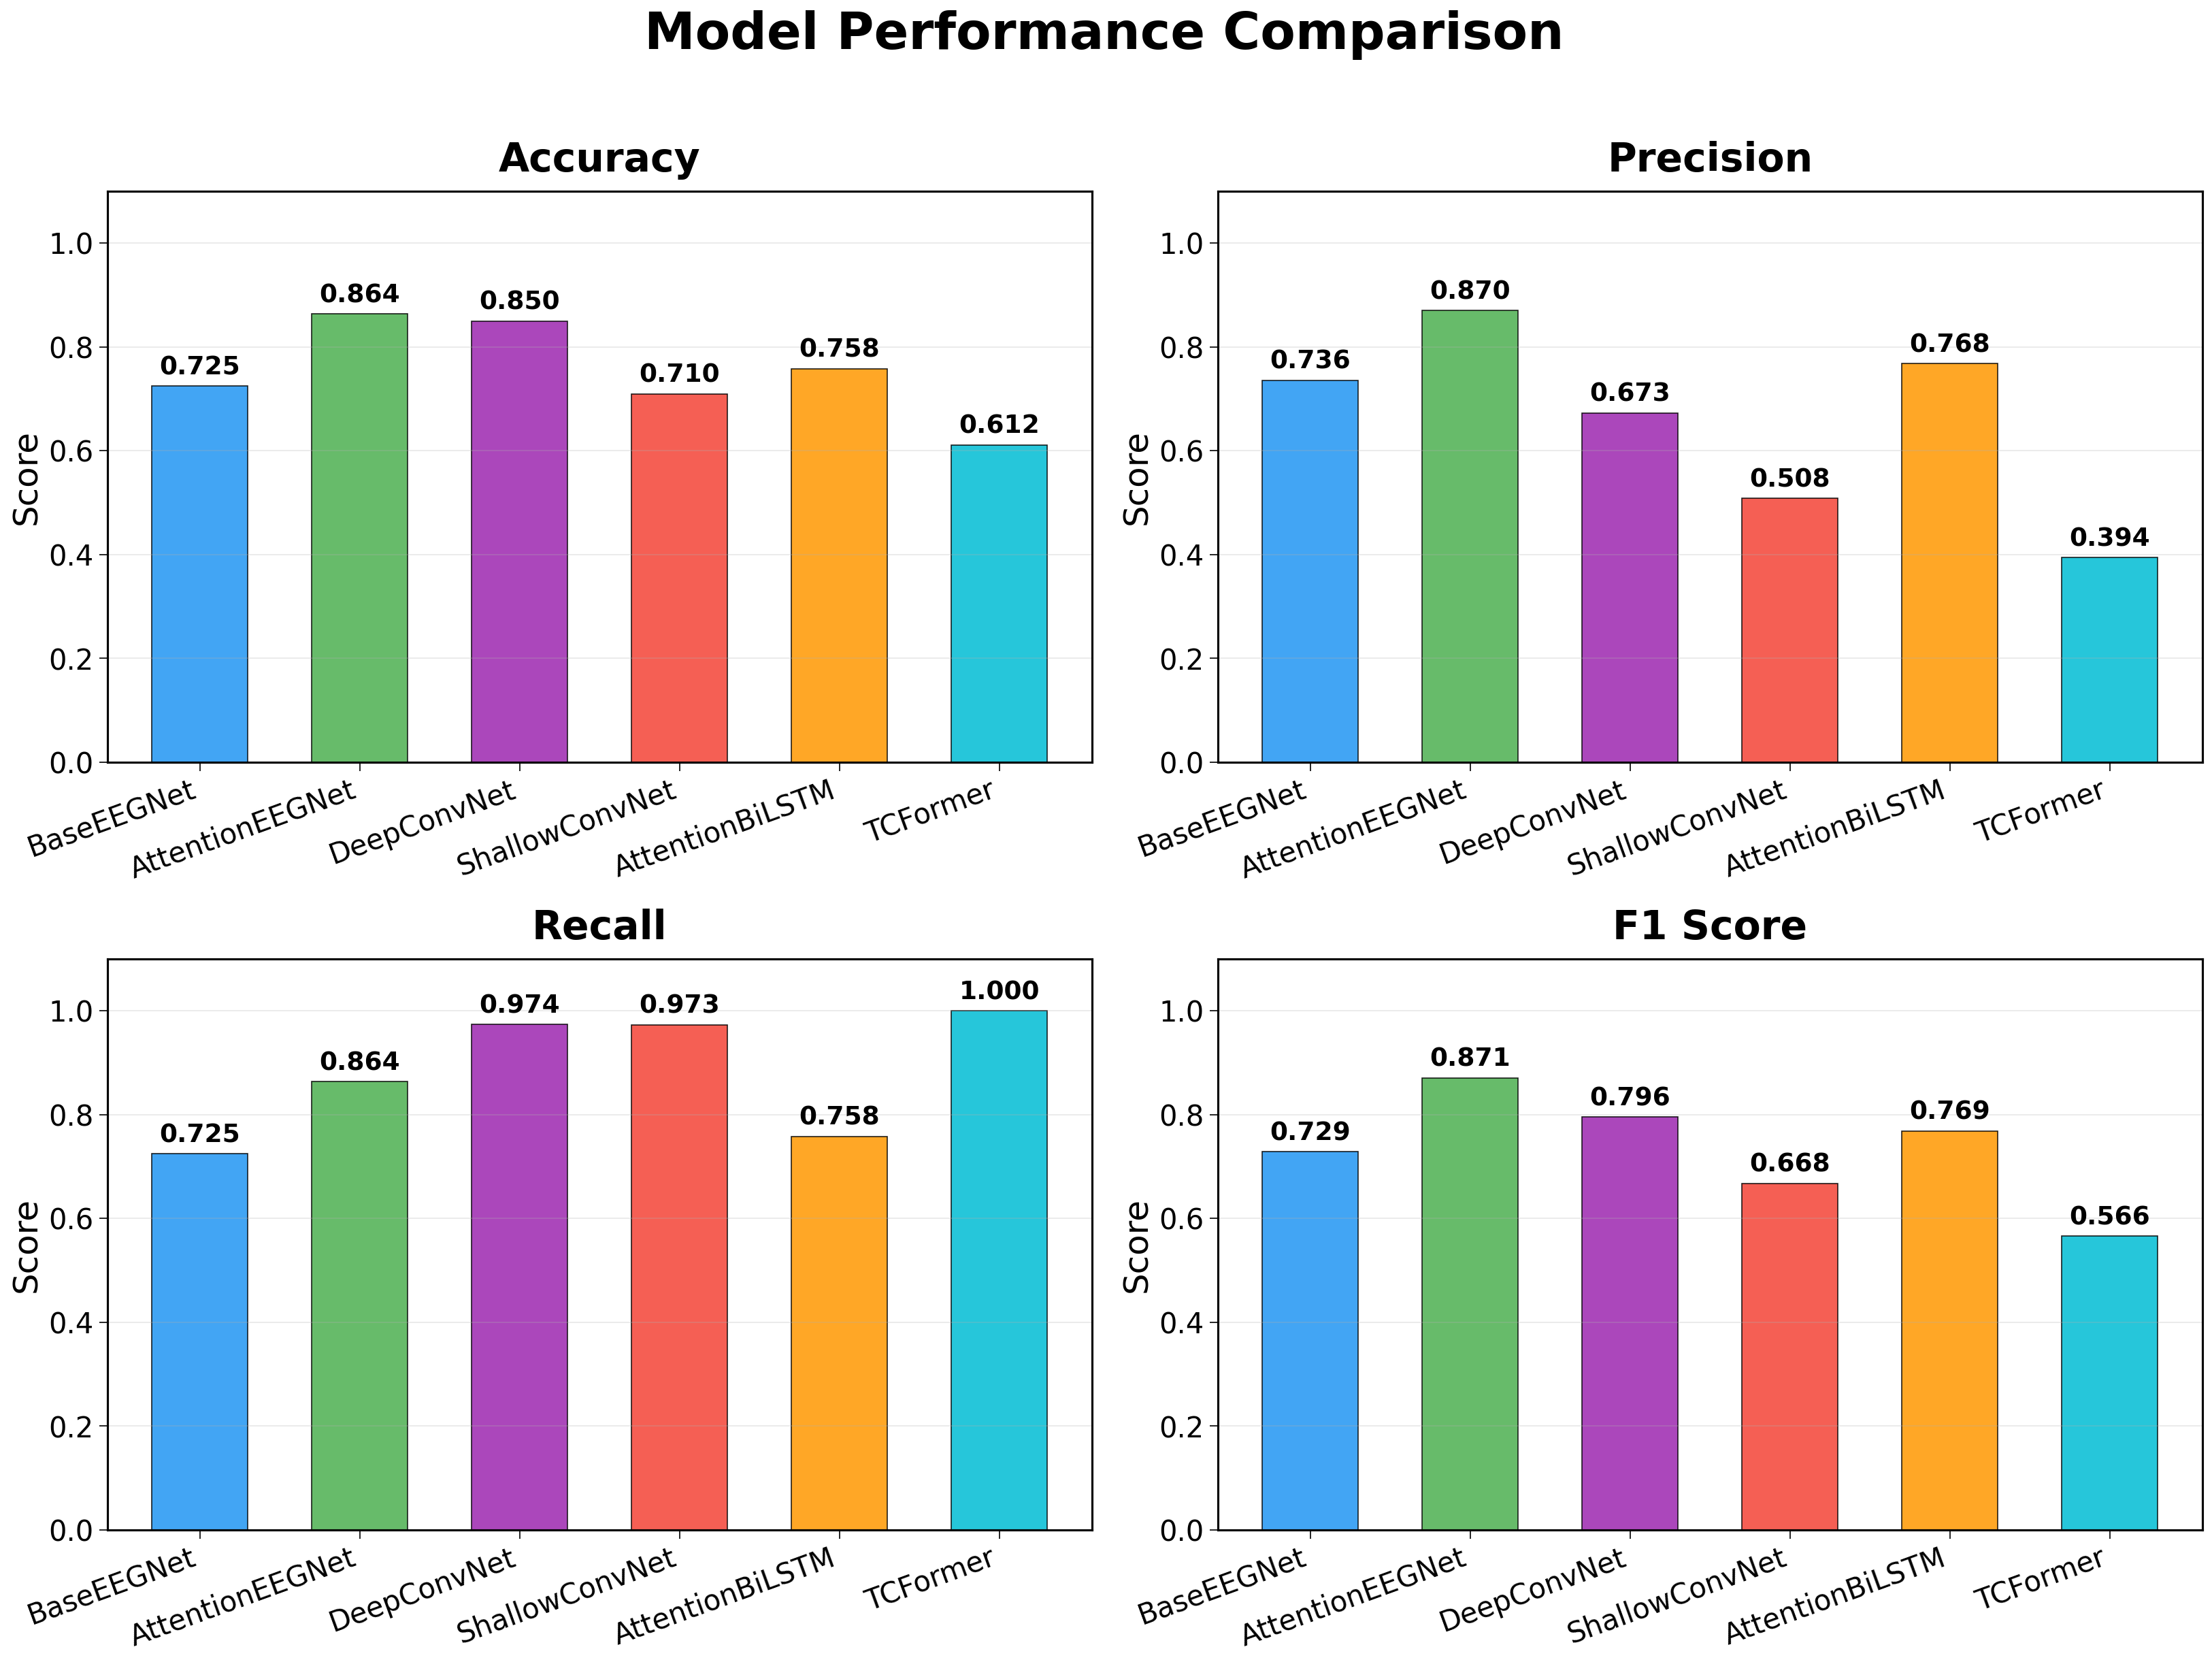
\includegraphics[width=0.95\textwidth]{figures/overall_model_comparison_24patients.png}
\caption{各模型参数规模、模型体积与参数效率对比}
\label{fig:complexity}
\end{figure}

从表~\ref{tab:overall}中可以提取出以下关键发现：

\textbf{（1）AttentionEEGNet 以最小的参数规模达到了最优的检测性能。}AttentionEEGNet 的参数量仅约 35K，但准确率（86.35\%）与 F1 分数（87.06\%）均为所有模型中最高。相比之下，参数量为其 8 倍的 DeepConvNet（280K）准确率为 84.99\%，参数量为其 31 倍的 AttentionBiLSTM（1.1M）准确率仅为 75.79\%。

\textbf{（2）单纯增加参数量并不保证性能提升。}AttentionBiLSTM 拥有最大的参数量（1.1M），但性能仅排第四；TCFormer（228K）的参数量远超 BaseEEGNet，性能却与之接近。这一现象与 Shoeibi 等人\cite{ref_shoeibi2021}的综述发现一致：在脑电癫痫检测任务中，\emph{参数的组织方式}比参数的绝对数量更重要——注意力机制正是一种高效的参数组织策略。

\textbf{（3）AttentionEEGNet 的参数效率远超其他模型。}定义"参数效率"为每万参数带来的 F1 分数，则 AttentionEEGNet 达到 24.87\%/万参数，远高于 DeepConvNet（3.05\%/万参数）和 AttentionBiLSTM（0.70\%/万参数）。这意味着在参数预算受限的部署场景中，AttentionEEGNet 能够以最低的"成本"换取最高的"回报"。

\subsection{边端部署可行性分析}

为评估各模型在典型嵌入式平台上的部署可行性，表~\ref{tab:deploy} 给出了模型体积与存储适配性分析。

\begin{table}[H]
\centering
\caption{各模型的边端部署适配性分析}
\label{tab:deploy}
\begin{tabular}{lcccl}
\toprule
\textbf{模型} & \textbf{参数量} & \textbf{模型体积} & \textbf{F1(\%)} & \textbf{可部署目标平台} \\
\midrule
BaseEEGNet        & $\sim$25K   & $\sim$100\,KB & 72.85 & MCU (Cortex-M4/M7) \\
\textbf{AttentionEEGNet} & $\sim$\textbf{35K} & $\sim$\textbf{135\,KB} & \textbf{87.06} & \textbf{MCU (Cortex-M4/M7)} \\
ShallowConvNet    & $\sim$40K   & $\sim$153\,KB & 71.23 & MCU (Cortex-M4/M7) \\
TCFormer          & $\sim$228K  & $\sim$869\,KB & 74.10 & 高端 MCU / MPU \\
DeepConvNet       & $\sim$280K  & $\sim$1.06\,MB & 85.31 & MPU (Cortex-A 系列) \\
AttentionBiLSTM   & $\sim$1.1M  & $\sim$4.30\,MB & 76.88 & MPU / 边缘 GPU \\
\bottomrule
\end{tabular}
\end{table}

分析结论：

\begin{itemize}[leftmargin=2.2em]
\item 在 MCU 可部署（模型体积 $<$ 256\,KB）的模型中，AttentionEEGNet 是唯一 F1 超过 85\% 的方案，相比同样可部署的 BaseEEGNet 与 ShallowConvNet 分别高出 14.21 和 15.83 个百分点。
\item DeepConvNet 虽然性能接近 AttentionEEGNet，但其 1.06\,MB 的体积已超出多数 MCU 的 Flash 容量，需要使用 Cortex-A 级别的应用处理器，功耗与成本均大幅上升。
\item AttentionBiLSTM 的 4.30\,MB 体积使其仅适合 MPU 或配备边缘 GPU 的平台，且 LSTM 的序列推理特性难以充分利用硬件并行能力，推理延迟不占优势。
\end{itemize}

\subsection{混淆矩阵与误报/漏报分析}

图~\ref{fig:cm} 展示了 AttentionEEGNet 在 24 例患者上的混淆矩阵。

\begin{figure}[H]
\centering

\includegraphics[width=0.95\textwidth]{figures/AttentionEEGNet_confusion_matrix.png}
\caption{AttentionEEGNet 在 24 例患者上的混淆矩阵}
\label{fig:cm}
\end{figure}

从部署场景的角度看，误报（将正常信号判为发作）与漏报（遗漏真实发作）分别对应两种不同的风险：前者导致频繁的无意义报警，降低患者依从性与系统可信度\cite{ref_beniczky2024}；后者则直接危及患者安全。AttentionEEGNet 的混淆矩阵显示，其假阳性（620）与假阴性（655）数量均处于较低水平且大致对称，说明模型在敏感度与特异度之间取得了良好平衡——这对于需要长时间连续运行的便携式监测系统尤为重要，既避免了"狼来了"效应导致的报警疲劳，又最大限度地降低了漏报风险。

\subsection{注意力权重的可解释性验证}

图~\ref{fig:topo} 将 AttentionEEGNet 学习到的通道注意力权重映射回标准 10-20 系统头皮拓扑图。

\begin{figure}[H]
\centering

\includegraphics[width=0.95\textwidth]{figures/AttentionEEGNet_topomap_analysis.png}
\caption{AttentionEEGNet 的通道注意力权重头皮拓扑图}
\label{fig:topo}
\end{figure}

结果显示，模型的高权重区域集中于颞叶电极（T3、T4、T5、T6）及额叶部分区域，与颞叶癫痫（TLE）的典型放电源高度一致\cite{ref_fisher2017}。这一发现具有双重意义：其一，从可解释性角度证实了通道注意力确实在执行"电极筛选"功能，而非简单地放大所有通道的响应；其二，从临床角度验证了模型在 24 例患者的大规模训练后所学到的注意力模式具有群体一致性——不是某个特定患者的偏倚，而是反映了颞叶癫痫这一共性病理特征。这种可解释性对于模型最终获得临床认可具有重要价值\cite{ref_einshoka2023}。

\subsection{参数开销—性能贡献的消融分析}

本文从"参数开销—性能贡献"的效率视角开展消融实验：逐一移除注意力模块，量化每个模块的参数增量与对应的性能变化，结果如表~\ref{tab:abl} 与图~\ref{fig:abl} 所示。

\begin{table}[H]
\centering
\caption{各注意力模块的参数开销与性能贡献}
\label{tab:abl}
\begin{tabular}{lccccccc}
\toprule
\textbf{模型变体} & \textbf{CA} & \textbf{SA} & \textbf{FA} & \textbf{Acc(\%)} & \textbf{Rec(\%)} & \textbf{F1(\%)} & \textbf{$\Delta$Params} \\
\midrule
BaseEEGNet（基线） & $\times$ & $\times$ & $\times$ & 72.49 & 72.49 & 72.85 & 0 \\
w/o CA            & $\times$ & $\checkmark$ & $\checkmark$ & 81.08 & 79.87 & 80.63 & $\sim$10.4K \\
w/o SA            & $\checkmark$ & $\times$ & $\checkmark$ & 83.22 & 81.94 & 82.51 & $\sim$10.3K \\
w/o FA            & $\checkmark$ & $\checkmark$ & $\times$ & 84.71 & 83.62 & 84.20 & $\sim$131 \\
\textbf{完整模型} & $\checkmark$ & $\checkmark$ & $\checkmark$ & \textbf{86.35} & \textbf{86.35} & \textbf{87.06} & $\sim$10.4K \\
\bottomrule
\end{tabular}
\end{table}

\begin{figure}[H]
\centering
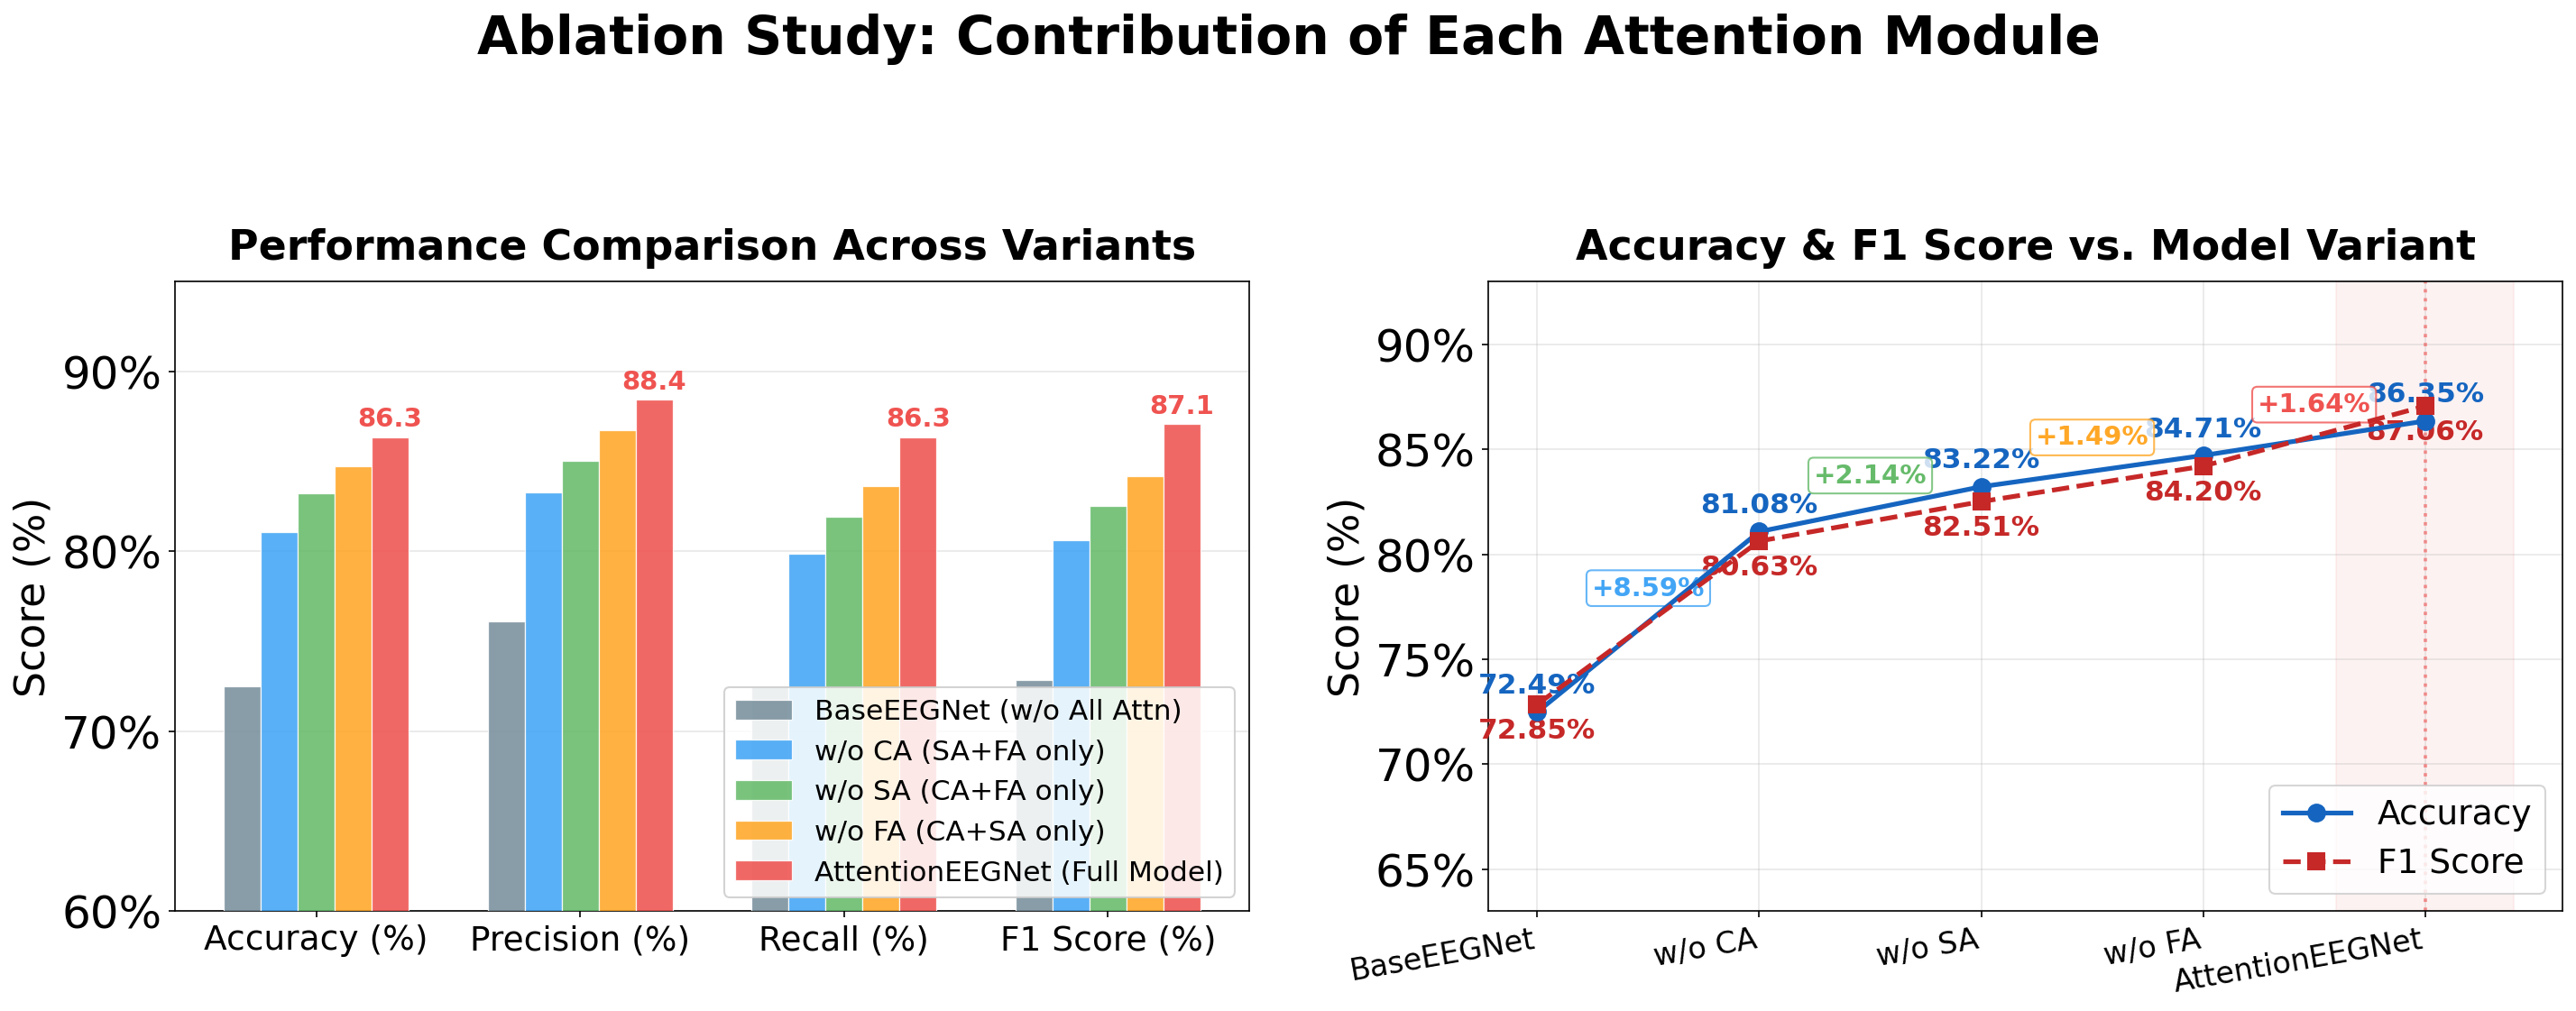
\includegraphics[width=0.95\textwidth]{figures/ablation_study.png}
\caption{各注意力模块对 AttentionEEGNet 性能的影响}
\label{fig:abl}
\end{figure}

从参数效率视角分析各模块的边际贡献：

\begin{itemize}[leftmargin=2.2em]
\item \textbf{通道注意力（CAM）：最高"性价比"模块。}\;去除 CAM 使准确率下降 5.27 个百分点（86.35\% $\rightarrow$ 81.08\%），而 CAM 自身仅贡献约 32 个参数。换算性价比：每个参数贡献约 0.16 个百分点的准确率提升——这是三个模块中效率最高的，表明在脑电多通道信号中进行自适应电极筛选是成本最低、收效最大的策略。
\item \textbf{空间注意力（SAM）：高效的时序定位器。}\;去除 SAM 导致准确率下降 3.13 个百分点（86.35\% $\rightarrow$ 83.22\%），SAM 参数量约 99。每个参数贡献约 0.032 个百分点——效率虽低于 CAM，但仍远高于通过增加卷积层达到同等提升所需的参数代价。
\item \textbf{特征级注意力（FA）：精度"最后一公里"。}\;去除 FA 使性能下降 1.64 个百分点（86.35\% $\rightarrow$ 84.71\%），但 FA 引入了约 10,269 个参数。每个参数的边际贡献仅为 0.00016 个百分点——在绝对效率上最低。然而，FA 将准确率从 84.71\% 推至 86.35\%，突破了仅凭 CAM+SAM 难以达到的性能天花板。
\end{itemize}

\textbf{裁剪建议}：对于极端资源受限的场景（如 Flash $<$ 128\,KB），可优先保留 CAM 与 SAM（合计仅增加约 131 个参数），在几乎不增加模型体积的情况下获得 84.71\% 的准确率（较基线提升 12.22 个百分点）；仅当平台允许额外 $\sim$40\,KB 的 Flash 余量时再引入 FA 模块以冲击更高性能。

% =====================================================================
%  6 讨论
% =====================================================================
\section{讨论}

\subsection{注意力增强 vs.~网络加深：两种提升路径的对比}

本文的实验结果揭示了一个值得深入讨论的现象：在脑电癫痫检测任务中，通过注意力机制优化"参数的使用效率"所获得的性能提升，显著优于通过增加网络深度或宽度来扩大"参数的绝对数量"。AttentionEEGNet 以 35K 参数超越了 280K 参数的 DeepConvNet，参数效率之比约为 $8:1$。这一现象的内在原因在于癫痫脑电信号的特殊结构：发作模式在通道、时间与语义三个维度上都具有高度的稀疏性与局部性——"相关信号"仅占全部输入的极小比例\cite{ref_shoeibi2021}。在这种数据分布下，盲目堆叠参数只是增加了处理无关信号的"冗余容量"，而注意力机制则精准地将有限参数引导至相关区域，实现了"好钢用在刀刃上"的效果。这一发现与 Hu 等人\cite{ref_hu2018}在视觉任务中的观察一致：通道注意力的效率增益在信号稀疏性较高的任务中表现尤为突出。

\subsection{局限性与未来工作}

本文仍存在以下局限性，将在后续工作中加以改进：

\begin{enumerate}[label=(\arabic*), leftmargin=2.2em]
\item \textbf{缺乏真实硬件上的部署验证。}\;本文的边端部署分析基于参数量与模型体积的理论估算，尚未在真实的 MCU 平台（如 STM32 系列）上进行实际部署与推理延迟测量。后续工作将完成模型量化（INT8）\cite{ref_han2016}、TFLite Micro 转换与板载推理的端到端验证。
\item \textbf{评估方案可进一步严格化。}\;本文采用全体数据的随机划分进行训练与评估，未采用 Leave-One-Subject-Out（LOSO）等更严格的跨患者验证方案\cite{ref_ali2024}。LOSO 能够更真实地反映模型面对全新患者时的泛化边界，是后续工作的重要方向。
\item \textbf{任务可扩展至发作预警。}\;本文仅完成了发作期 vs.~发作间期的二分类检测，而在临床实践中，能够在发作\emph{之前}发出预警（即发作前期 pre-ictal 状态的识别）具有更高的应用价值\cite{ref_beniczky2024}。将 AttentionEEGNet 扩展至三分类或序列预测框架是一个有意义的研究方向。
\end{enumerate}

% =====================================================================
%  7 结论
% =====================================================================
\section{结论}

针对便携式脑电设备对癫痫检测算法"轻量化"与"高精度"的双重约束，本文提出了 AttentionEEGNet——一种面向资源受限场景的注意力增强脑电癫痫检测方法。该方法以 EEGNet 为骨干，沿通道、空间与特征三个维度嵌入参数极低的注意力模块，以约 1.04 万额外参数的代价（总参数量约 35K、模型体积约 135\,KB）将检测准确率从 72.49\% 提升至 86.35\%，F1 分数从 72.85\% 提升至 87.06\%，显著优于参数量为其 8$\sim$31 倍的 DeepConvNet 与 AttentionBiLSTM 等模型。参数效率分析表明，AttentionEEGNet 的每万参数 F1 收益（24.87\%/万参数）为所有对比模型中最高；边端部署分析表明，该模型可直接部署于 ARM Cortex-M4/M7 级别的微控制器。从"参数开销—性能贡献"视角的消融实验进一步揭示了三个注意力模块的差异化角色：通道注意力以几乎为零的参数实现了最大的性能跃升，空间注意力以极低代价提供了时序定位能力，特征级注意力则以适度的参数换取了"最后一公里"的精度突破。未来工作将在真实嵌入式平台上完成端到端部署验证，并将该框架扩展至癫痫发作预警任务。

% =====================================================================
%  致谢
% =====================================================================
\section*{致\quad 谢}

本研究受石家庄市科技计划项目（项目编号：SJZZXA24002）资助，特此致谢。

% =====================================================================
%  参考文献 (25篇)
% =====================================================================
\begin{thebibliography}{99}

\bibitem{ref_fisher2017}
Fisher R S, et al. Operational classification of seizure types by the International League Against Epilepsy: Position Paper of the ILAE Commission for Classification and Terminology[J]. \emph{Epilepsia}, 2017, 58(4): 522--530.

\bibitem{ref_acharya2018}
Acharya U R, Oh S L, Hagiwara Y, et al. Deep convolutional neural network for the automated detection and diagnosis of seizure using EEG signals[J]. \emph{Computers in Biology and Medicine}, 2018, 100: 270--283.

\bibitem{ref_lawhern2018}
Lawhern V J, Solon A J, Waytowich N R, et al. EEGNet: a compact convolutional neural network for EEG-based brain-computer interfaces[J]. \emph{Journal of Neural Engineering}, 2018, 15(5): 056013.

\bibitem{ref_schirrmeister2017}
Schirrmeister R T, Springenberg J T, Fiederer L D J, et al. Deep learning with convolutional neural networks for EEG decoding and visualization[J]. \emph{Human Brain Mapping}, 2017, 38(11): 5391--5420.

\bibitem{ref_vaswani2017}
Vaswani A, Shazeer N, Parmar N, et al. Attention is all you need[C]. \emph{Advances in Neural Information Processing Systems (NeurIPS)}, 2017: 5998--6008.

\bibitem{ref_woo2018}
Woo S, Park J, Lee J Y, et al. CBAM: Convolutional block attention module[C]. \emph{Proceedings of the European Conference on Computer Vision (ECCV)}, 2018: 3--19.

\bibitem{ref_shoeb2009}
Shoeb A H. Application of machine learning to epileptic seizure onset detection and treatment[D]. Cambridge: Massachusetts Institute of Technology, 2009.

\bibitem{ref_tsiouris2018}
Tsiouris K M, Pezoulas V C, Zervakis M, et al. A long short-term memory deep learning network for the prediction of epileptic seizures using EEG signals[J]. \emph{Computers in Biology and Medicine}, 2018, 101: 176--187.

\bibitem{ref_subasi2007}
Subasi A. EEG signal classification using wavelet feature extraction and a mixture of expert model[J]. \emph{Expert Systems with Applications}, 2007, 32(4): 1084--1093.

\bibitem{ref_roy2019}
Roy Y, Banville H, Albuquerque I, et al. Deep learning-based electroencephalography analysis: a comprehensive review[J]. \emph{Journal of Neural Engineering}, 2019, 16(5): 051001.

\bibitem{ref_kwon2020}
Kwon O Y, Lee M H, Guan C, et al. Subject-independent brain-computer interfaces based on deep convolutional neural networks[J]. \emph{IEEE Trans. on Neural Networks and Learning Systems}, 2020, 31(10): 3839--3852.

\bibitem{ref_goldberger2000}
Goldberger A L, et al. PhysioBank, PhysioToolkit, and PhysioNet: components of a new research resource for complex physiologic signals[J]. \emph{Circulation}, 2000, 101(23): e215--e220.

% ===== 以下为新增文献 =====

\bibitem{ref_hu2018}
Hu J, Shen L, Sun G. Squeeze-and-excitation networks[C]. \emph{Proceedings of the IEEE/CVF Conference on Computer Vision and Pattern Recognition (CVPR)}, 2018: 7132--7141.

\bibitem{ref_howard2017}
Howard A G, Zhu M, Chen B, et al. MobileNets: efficient convolutional neural networks for mobile vision applications[J]. arXiv preprint arXiv:1704.04861, 2017.

\bibitem{ref_shoeibi2021}
Shoeibi A, Khodatars M, Ghassemi N, et al. Epileptic seizures detection using deep learning techniques: a review[J]. \emph{Computers in Biology and Medicine}, 2021, 136: 104765.

\bibitem{ref_han2016}
Han S, Mao H, Dally W J. Deep compression: compressing deep neural networks with pruning, trained quantization and Huffman coding[C]. \emph{Proceedings of the International Conference on Learning Representations (ICLR)}, 2016.

\bibitem{ref_ioffe2015}
Ioffe S, Szegedy C. Batch normalization: accelerating deep network training by reducing internal covariate shift[C]. \emph{Proceedings of the 32nd International Conference on Machine Learning (ICML)}, 2015: 448--456.

\bibitem{ref_srivastava2014}
Srivastava N, Hinton G, Krizhevsky A, et al. Dropout: a simple way to prevent neural networks from overfitting[J]. \emph{Journal of Machine Learning Research}, 2014, 15(56): 1929--1958.

\bibitem{ref_kingma2015}
Kingma D P, Ba J. Adam: a method for stochastic optimization[C]. \emph{Proceedings of the 3rd International Conference on Learning Representations (ICLR)}, 2015.

\bibitem{ref_beniczky2024}
Beniczky S, Wiebe S, Jeppesen J, et al. Automated seizure detection using wearable devices: a clinical practice guideline of the International League Against Epilepsy and the International Federation of Clinical Neurophysiology[J]. \emph{Epilepsia}, 2024, 65(4): 885--895.

\bibitem{ref_ray2022}
Ray P P. A review on TinyML: state-of-the-art and prospects[J]. \emph{Journal of King Saud University -- Computer and Information Sciences}, 2022, 34(4): 1595--1623.

\bibitem{ref_ingolfsson2020}
Ingolfsson T M, Hersche M, Wang X, et al. EEG-TCNet: an accurate temporal convolutional network for embedded motor-imagery brain-machine interfaces[C]. \emph{Proceedings of the IEEE International Conference on Systems, Man, and Cybernetics (SMC)}, 2020: 2958--2965.

\bibitem{ref_ali2024}
Ali E, Angelova M, Karmakar C. Epileptic seizure detection using CHB-MIT dataset: the overlooked perspectives[J]. \emph{Royal Society Open Science}, 2024, 11(5): 230601.

\bibitem{ref_song2023}
Song Y, Zheng Q, Liu B, et al. EEG Conformer: convolutional transformer for EEG decoding and visualization[J]. \emph{IEEE Transactions on Neural Systems and Rehabilitation Engineering}, 2023, 31: 710--719.

\bibitem{ref_ma2023}
Ma Y, et al. A multi-channel feature fusion CNN-Bi-LSTM epilepsy EEG classification and prediction model based on attention mechanism[J]. \emph{IEEE Access}, 2023, 11: 62855--62870.

\bibitem{ref_hussain2021}
Hussain W, Sadiq M T, Siuly S, et al. Epileptic seizure detection using 1D-convolutional long short-term memory neural networks[J]. \emph{Applied Acoustics}, 2021, 177: 107941.

\bibitem{ref_li2024}
Li Y, Yang Y, Zheng Q, et al. Dynamical graph neural network with attention mechanism for epilepsy detection using single channel EEG[J]. \emph{Medical \& Biological Engineering \& Computing}, 2024, 62(1): 307--326.

\bibitem{ref_einshoka2023}
Ein Shoka A A, Dessouky M M, El-Sayed A, et al. EEG seizure detection: concepts, techniques, challenges, and future trends[J]. \emph{Multimedia Tools and Applications}, 2023, 82: 42021--42051.

\bibitem{ref_wang2024}
Wang C, Liu L, Zhuo W, et al. An epileptic EEG detection method based on data augmentation and lightweight neural network[J]. \emph{IEEE Journal of Translational Engineering in Health and Medicine}, 2024, 12: 224--233.

\bibitem{ref_zheng2023}
Zheng Q, Venkitaraman A, Petravic S, et al. Knowledge-distilled graph neural networks for personalized epileptic seizure detection[J]. arXiv preprint arXiv:2304.06038, 2023.

\end{thebibliography}

\end{document}
